\documentclass{beamer}


\mode<presentation>
{
  \usetheme{CambridgeUS}
	\usecolortheme{beaver}
  % or ...

  \setbeamercovered{transparent}
  % or whatever (possibly just delete it)
}


\usepackage{xeCJK}
\usepackage{ulem}
\usepackage[english]{babel}
\usepackage[utf8]{inputenc}
\usepackage{times}
\usepackage[T1]{fontenc}
\usepackage{hyperref}
\usepackage{pifont}
\usepackage{biblatex}
\usepackage{bibentry}
\usepackage{verbatim}
\usepackage{listings}
\bibliography{cite}
\newcommand{\cmark}{\ding{51}}%
\newcommand{\xmark}{\ding{55}}%
\setCJKmainfont{WenQuanYi Micro Hei}
\renewcommand{\raggedright}{\leftskip=0pt \rightskip=0pt plus 0cm}
\raggedright

\let\oldfootnotesize\footnotesize
\renewcommand*{\footnotesize}{\oldfootnotesize\tiny}

\title[Intelligent Software Engineering] 
{Intelligent Software Engineering}
\subtitle{Introduction to Artificial Intelligence}

\author[Zhilei Ren] 
{Zhilei Ren}

\institute[Dalian University of Technology] % (optional, but mostly needed)
{
\\
\includegraphics[width=0.1\textwidth]{../utils/logo.png}\\
Dalian University of Technology
}


\subject{Software Engineering}



\pgfdeclareimage[width=0.08\textwidth]{university-logo}{../utils/logo.png}
\logo{\pgfuseimage{university-logo}}



% Delete this, if you do not want the table of contents to pop up at
% the beginning of each subsection:
\AtBeginSubsection[]
{
  \begin{frame}<beamer>{Outline}
    \tableofcontents[currentsection,currentsubsection]
  \end{frame}
}


% If you wish to uncover everything in a step-wise fashion, uncomment
% the following command: 

%\beamerdefaultoverlayspecification{<+->}

\setbeamertemplate{section in toc}[circle]
\setbeamertemplate{items}[circle]
\setbeamertemplate{caption}[numbered]
\setbeamertemplate{bibliography item}{\insertbiblabel}
\setbeamertemplate{bibliography entry title}{}
\setbeamertemplate{bibliography entry journal}{}

% PlantUML listing configuration
\lstdefinestyle{plantuml}{
    language=Java,
    basicstyle=\ttfamily\small,
    keywordstyle=\color{blue},
    commentstyle=\color{green!60!black},
    stringstyle=\color{red},
    numbers=left,
    numberstyle=\tiny\color{gray},
    stepnumber=1,
    numbersep=5pt,
    backgroundcolor=\color{white!95!black},
    frame=single,
    rulecolor=\color{black},
    tabsize=2,
    captionpos=b,
    breaklines=true,
    breakatwhitespace=false,
    showstringspaces=false
}

\begin{document}

\begin{frame}
  \titlepage
\end{frame}

\begin{frame}{Outline}
  \tableofcontents[currentsection,currentsubsection, 
    sectionstyle=show,
    subsectionstyle=show,
]
\end{frame}

\AtBeginSubsection[]
{
  \begin{frame}<beamer>{Outline}
    \tableofcontents[currentsection,currentsubsection]
  \end{frame}
}

\begin{frame}[t]{Vibe Coding}
    Vibe coding is an artificial intelligence-assisted software development style popularized by Andrej Karpathy in February 2025. The term was listed in the Merriam-Webster Dictionary the following month as a ``slang \& trending'' term. It describes a chatbot-based approach to creating software where the developer describes a project or task to a large language model (LLM), which generates code based on the prompt. The developer evaluates the result and asks the LLM for improvements. Unlike traditional AI-assisted coding or pair programming, the human developer avoids micromanaging the code, accepts AI-suggested completions liberally, and focuses more on iterative experimentation than code correctness or structure\footnote{\url{https://en.wikipedia.org/wiki/Vibe_coding}}.
\end{frame}

\begin{frame}[t]{The Illusion of AI Productivity}
    \centering
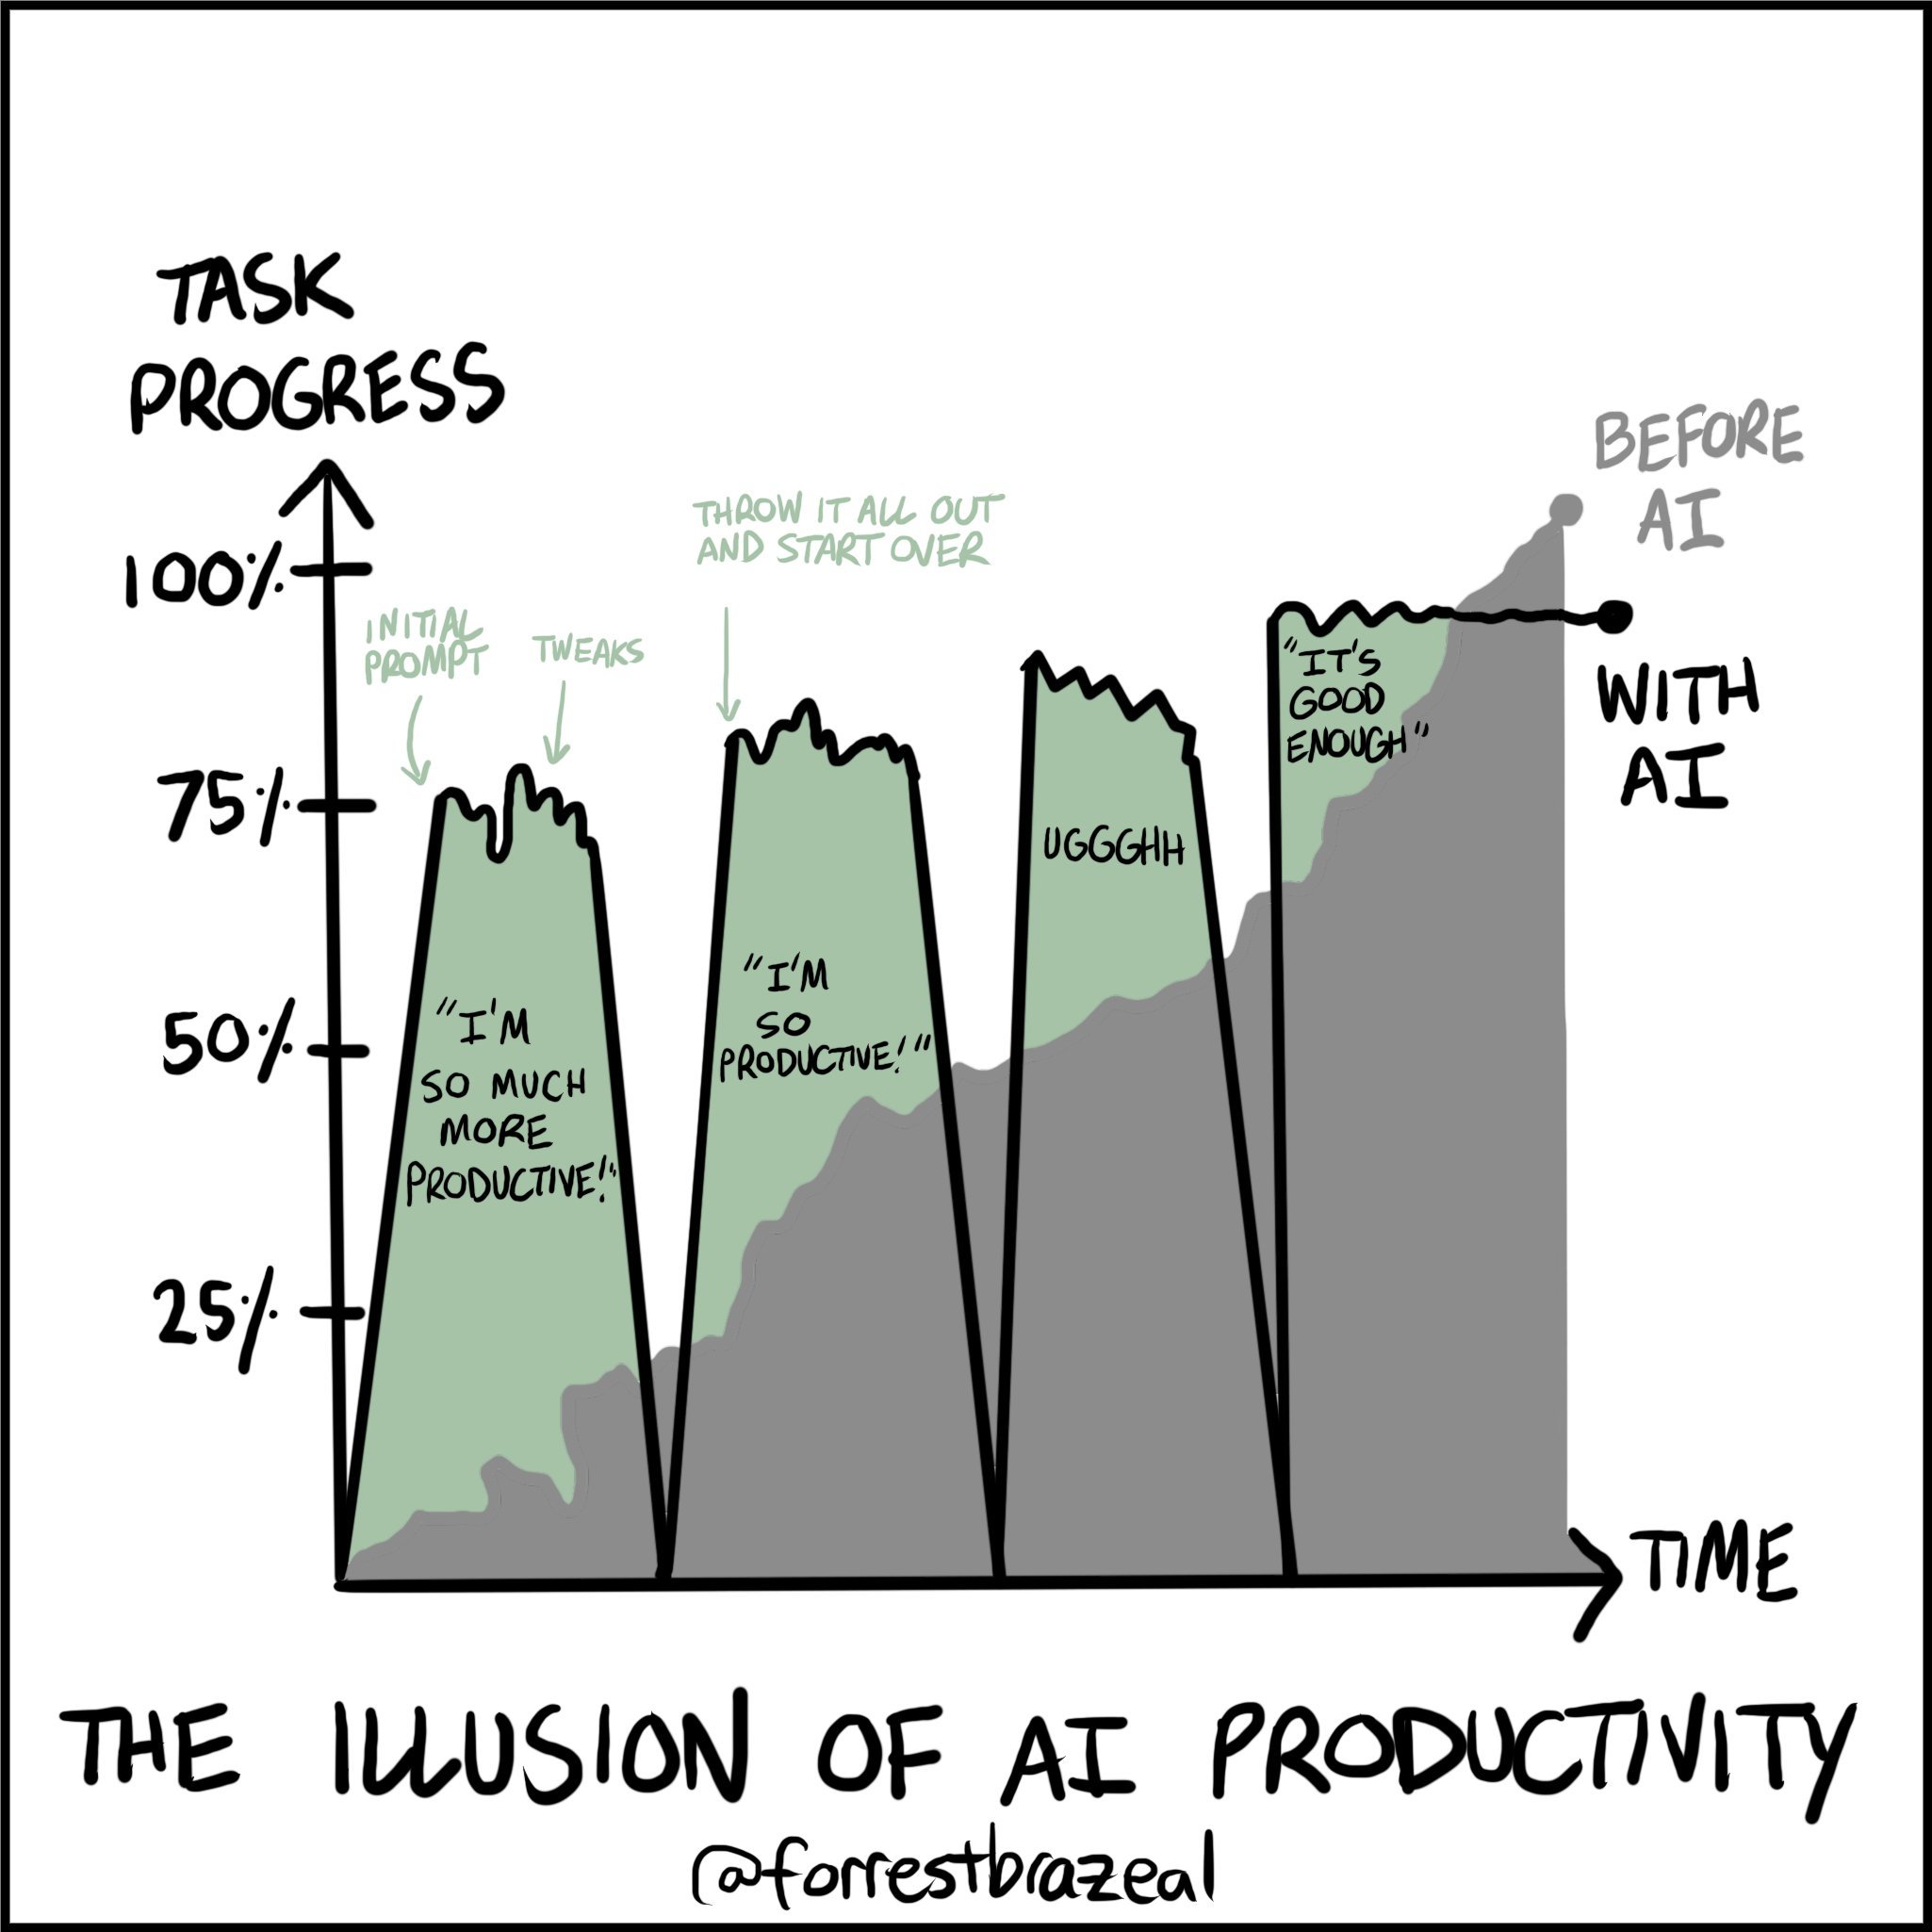
\includegraphics[width=.5\textwidth]{before_ai.jpeg} 
\end{frame}

\section{Introduction}
\begin{frame}[t]{Intelligent Software Engineering}
\begin{itemize}
\item \textbf{Beyond Traditional Methods}: AI and optimization techniques in software development
\item \textbf{Multiple Approaches}: Different intelligent methods for different problems
\item \textbf{Complementary Strengths}: Each method excels in specific domains
\item \textbf{Practical Applications}: Real-world tools and techniques used today
\item \textbf{Human-AI Collaboration}: Augmenting developer capabilities
\end{itemize}
\end{frame}

\section{Intelligent Methods Overview}
\begin{frame}[t]{Spectrum of Intelligent Approaches}
\begin{itemize}
\item \textbf{LLM-based Methods}: Natural language understanding and generation
\item \textbf{Search-based Optimization}: Evolutionary algorithms and local search
\item \textbf{Constraint Solving}: Formal methods and SAT solving
\item \textbf{Hybrid Approaches}: Combining multiple intelligent techniques
\item \textbf{Specialized AI}: Domain-specific machine learning models
\end{itemize}
\begin{figure}
\includegraphics[width=0.6\textwidth]{example-image}
\caption{Intelligent methods landscape in software engineering}
\end{figure}
\end{frame}

\section{Large Language Models (LLMs)}
\begin{frame}[t]{LLM-based Approaches}
\begin{itemize}
\item \textbf{Foundation}: Transformer architecture trained on massive text/code corpora
\item \textbf{Strengths}: Natural language understanding, code generation, documentation
\item \textbf{Applications}: Code completion, architecture design, API generation
\item \textbf{Examples}: GitHub Copilot, ChatGPT, CodeLlama
\item \textbf{Limitations}: Hallucinations, lack of formal guarantees
\end{itemize}
\end{frame}

\begin{frame}[fragile,t]{LLM Code Implementation Example}
\begin{verbatim}
// Prompt: "Implement a thread-safe LRU cache in Java"
public class LRUCache<K, V> {
    private final int capacity;
    private final LinkedHashMap<K, V> cache;
    
    public LRUCache(int capacity) {
        this.capacity = capacity;
        this.cache = new LinkedHashMap<K, V>(
            capacity, 0.75f, true) {
            protected boolean removeEldestEntry(
                Map.Entry<K, V> eldest) {
                return size() > capacity;
            }
        };
    }
    // Additional methods implemented by LLM...
}
\end{verbatim}
\end{frame}

\section{Search-Based Software Engineering}
\begin{frame}[t]{SBSE for Software Design and Implementation}
\begin{itemize}
\item \textbf{Foundation}: Treat software design as search problem in solution space
\item \textbf{Strengths}: Finding optimal or near-optimal design solutions
\item \textbf{Applications}: Algorithm selection, data structure optimization, code synthesis
\item \textbf{Key Insight}: Software design decisions can be optimized systematically
\end{itemize}
\end{frame}

\begin{frame}[t]{SBSE for Algorithm Selection and Implementation}
\begin{itemize}
\item \textbf{Problem}: Choose optimal algorithm for specific problem constraints
\item \textbf{Search Space}: Different algorithms and their parameterizations
\item \textbf{Fitness Function}: Runtime complexity, memory usage, implementation complexity
\item \textbf{Method}: Genetic algorithm exploring algorithm combinations
\item \textbf{Result}: Best algorithm choice with optimized parameters
\end{itemize}
\begin{figure}
\includegraphics[width=0.4\textwidth]{example-image}
\caption{Algorithm selection search space}
\end{figure}
\end{frame}

\begin{frame}[fragile,t]{SBSE for Data Structure Optimization}
\begin{verbatim}
// Problem: Optimize data structure for frequent insertions and rare lookups
// Search-based approach explores different data structure implementations

// Candidate solutions explored:
Solution 1: ArrayList with binary search (O(n) insert, O(log n) lookup)
Solution 2: LinkedList (O(1) insert, O(n) lookup)  
Solution 3: Balanced BST (O(log n) insert, O(log n) lookup)
Solution 4: Hash table with lazy deletion (O(1) insert, O(1) lookup)

// Fitness evaluation based on actual usage patterns
// Optimal solution selected: LinkedList for 90% insert-heavy workload
\end{verbatim}
\end{frame}

\begin{frame}[t]{SBSE for Code Synthesis and Completion}
\begin{itemize}
\item \textbf{Challenge}: Automatically complete partial code implementations
\item \textbf{Approach}: Genetic programming with code fragments as building blocks
\item \textbf{Fitness}: Type correctness, test case passing, code quality metrics
\item \textbf{Application}: Auto-completing complex algorithmic implementations
\item \textbf{Example}: Synthesizing efficient matrix operations from specifications
\end{itemize}
\end{frame}

\begin{frame}[fragile,t]{SBSE for API Implementation Completion}
\begin{verbatim}
// Partial implementation provided by developer
public interface DataProcessor {
    Data process(Input input);
    // Additional methods to be completed...
}

// SBSE generates complete implementation based on usage patterns
public class EfficientDataProcessor implements DataProcessor {
    public Data process(Input input) { /* optimized */ }
    public void validate(Data data) { /* auto-generated */ }
    public Result batchProcess(List<Input> inputs) { /* synthesized */ }
    // Additional methods synthesized by search-based approach
}
\end{verbatim}
\end{frame}

\section{Constraint-Based Methods}
\begin{frame}[t]{Constraint Solving for Software Design}
\begin{itemize}
\item \textbf{Foundation}: Encode design constraints as logical formulas
\item \textbf{Strengths}: Guaranteed satisfaction of specified properties
\item \textbf{Applications}: Type-driven synthesis, interface conformance, design patterns
\item \textbf{Key Benefit}: Formal verification of design decisions
\end{itemize}
\end{frame}

\begin{frame}[t]{Constraint-Based API Design and Implementation}
\begin{itemize}
\item \textbf{Problem}: Ensure API consistency and completeness
\item \textbf{Constraints}: Method preconditions, postconditions, invariants
\item \textbf{Method}: Enforce constraints during API evolution
\item \textbf{Application}: Automated checking of API design rules
\item \textbf{Benefit}: Early detection of design violations
\end{itemize}
\begin{figure}
\includegraphics[width=0.5\textwidth]{example-image}
\caption{Constraint-based API verification}
\end{figure}
\end{frame}

\begin{frame}[fragile,t]{Constraint-Based Code Completion}
\begin{verbatim}
// Partial code with type constraints
public <T> T process(List<T> items) {
    // Constraint solver infers missing operations
    // Constraints: T must support comparison, serialization
    // Based on usage context and method signatures
    
    // Solution generated by constraint solver:
    Collections.sort(items);  // T must implement Comparable
    return serializer.serialize(items); // T must be serializable
}

// Constraint solver ensures type safety and API consistency
\end{verbatim}
\end{frame}

\begin{frame}[t]{Constraint-Based Design Pattern Implementation}
\begin{itemize}
\item \textbf{Objective}: Correctly implement design patterns with formal guarantees
\item \textbf{Constraints}: Pattern-specific rules (Observer: subject-observer relationships)
\item \textbf{Method}: Encode pattern constraints as logical formulas
\item \textbf{Verification}: Check implementation against pattern constraints
\item \textbf{Completion}: Suggest missing pattern elements
\end{itemize}
\end{frame}

\begin{frame}[fragile,t]{Constraint-Based Singleton Pattern Enforcement}
\begin{verbatim}
// Constraint: Singleton class must have private constructor
// and static getInstance method

class DatabaseConnection {
    private static DatabaseConnection instance;
    
    // Constraint solver verifies:
    // ✓ Constructor is private
    // ✓ getInstance method exists and is static
    // ✓ Instance variable is static
    
    private DatabaseConnection() {}  // Verified: private
    public static DatabaseConnection getInstance() { // Verified: static
        if (instance == null) {
            instance = new DatabaseConnection();
        }
        return instance;
    }
}
\end{verbatim}
\end{frame}

\section{Natural Language Processing}
\begin{frame}[t]{NLP for Design Specification Processing}
\begin{itemize}
\item \textbf{Foundation}: Extract design intent from natural language
\item \textbf{Strengths}: Bridging requirement documents and implementation
\item \textbf{Applications}: Design pattern recognition, architecture extraction
\item \textbf{Evolution}: From manual analysis to automated understanding
\end{itemize}
\end{frame}

\section{Hybrid Approaches}
\begin{frame}[t]{Combining Methods for Design and Implementation}
\begin{itemize}
\item \textbf{LLM + Constraints}: Generate code with formal verification
\item \textbf{SBSE + Constraints}: Search with guaranteed constraint satisfaction
\item \textbf{NLP + SBSE}: Extract design constraints for optimization
\item \textbf{Multi-method Integration}: Comprehensive design assistance
\end{itemize}
\begin{figure}
\includegraphics[width=0.5\textwidth]{example-image}
\caption{Hybrid intelligent design system}
\end{figure}
\end{frame}

\begin{frame}[fragile,t]{Hybrid Example: Intelligent Code Completion}
\begin{verbatim}
// Developer writes partial method:
public String processData(String input) {
    // Step 1: LLM suggests initial completion
    if (input == null) return "";
    String result = input.trim();
    
    // Step 2: Constraint solver verifies null safety
    // ✓ input checked for null, ✓ return value not null
    
    // Step 3: SBSE optimizes string operations
    // Replaces inefficient concatenation with StringBuilder
    
    // Step 4: Final verified and optimized code
    StringBuilder sb = new StringBuilder();
    sb.append(result.toLowerCase());
    return sb.toString();
}
\end{verbatim}
\end{frame}

\section{Application Domains}
\begin{frame}[t]{Software Design and Implementation}
\begin{itemize}
\item \textbf{LLMs}: Rapid prototyping and boilerplate generation
\item \textbf{SBSE}: Optimal algorithm and data structure selection
\item \textbf{Constraint-based}: Type-safe API design and implementation
\item \textbf{Hybrid}: End-to-end design and implementation assistance
\end{itemize}
\end{frame}

\begin{frame}[t]{Code Completion and Synthesis}
\begin{itemize}
\item \textbf{LLMs}: Context-aware code suggestions
\item \textbf{SBSE}: Optimization-driven completion
\item \textbf{Constraint-based}: Type-directed synthesis with guarantees
\item \textbf{NLP}: Requirement-driven implementation
\end{itemize}
\end{frame}

\begin{frame}[t]{Architecture and Pattern Implementation}
\begin{itemize}
\item \textbf{Constraint-based}: Formal pattern verification
\item \textbf{SBSE}: Optimal pattern instantiation
\item \textbf{LLMs}: Pattern explanation and examples
\item \textbf{Hybrid}: Pattern-compliant architecture generation
\end{itemize}
\end{frame}

\section{Comparative Analysis}
\begin{frame}[t]{Method Comparison for Design/Implementation}
\begin{center}
\begin{tabular}{lccc}
\textbf{Method} & \textbf{Correctness Guarantees} & \textbf{Creativity} & \textbf{Speed} \\
\hline
LLM-based & Low & High & Fast \\
SBSE & Medium & Medium & Medium \\
Constraint-based & High & Low & Slow \\
Hybrid & High & High & Medium \\
\end{tabular}
\end{center}

\begin{itemize}
\item \textbf{Correctness Guarantees}: Formal verification capabilities
\item \textbf{Creativity}: Novel solution generation
\item \textbf{Speed}: Response time for practical use
\end{itemize}
\end{frame}

\begin{frame}[t]{Strengths for Design and Implementation}
\begin{itemize}
\item \textbf{LLMs}: Excellent for exploratory design and rapid prototyping
\item \textbf{SBSE}: Superior for optimization problems and algorithm selection
\item \textbf{Constraint-based}: Unmatched for correctness-critical components
\item \textbf{Hybrid}: Balanced approach for complex design challenges
\end{itemize}
\end{frame}

\section{Tools and Frameworks}
\begin{frame}[t]{Design and Implementation Tools}
\begin{itemize}
\item \textbf{LLM-based}: GitHub Copilot, Amazon CodeWhisperer, Tabnine
\item \textbf{SBSE}: Program synthesis tools (SKETCH, Rosette)
\item \textbf{Constraint-based}: Z3 for program verification, Alloy for design
\item \textbf{Hybrid}: Intelligent IDEs with multiple AI assistants
\end{itemize}
\end{frame}

\section{Future Directions}
\begin{frame}[t]{Emerging Trends in Intelligent Development}
\begin{itemize}
\item \textbf{Automated Design Synthesis}: From requirements to implementation
\item \textbf{Context-Aware Completion}: Understanding project-specific patterns
\item \textbf{Real-time Design Validation}: Continuous constraint checking
\item \textbf{Personalized Code Generation}: Adapting to individual coding styles
\item \textbf{Multi-modal Design Tools}: Combining code, diagrams, and specifications
\end{itemize}
\end{frame}

\section{Best Practices}
\begin{frame}[t]{Effective Intelligent Design Assistance}
\begin{itemize}
\item \textbf{Problem-Solution Fit}: Match method to design challenge characteristics
\item \textbf{Incremental Adoption}: Start with well-defined subproblems
\item \textbf{Validation Strategy}: Always verify intelligent system outputs
\item \textbf{Human Oversight}: Maintain designer control and understanding
\item \textbf{Documentation}: Record AI-assisted design decisions and rationale
\end{itemize}
\end{frame}

\begin{frame}[t]{Conclusion}
\begin{itemize}
\item \textbf{Rich Methodology}: Diverse intelligent approaches for software design
\item \textbf{Practical Value}: Accelerating and improving design decisions
\item \textbf{Complementary Nature}: Different methods excel at different tasks
\item \textbf{Human-Centric}: Augmenting rather than replacing designers
\item \textbf{Rapid Evolution}: Continuous improvement in intelligent assistance
\end{itemize}

\vspace{0.5cm}
\textbf{Key Insight}: Intelligent methods provide powerful assistance for complex software design and implementation challenges
\end{frame}

\begin{frame}[t]
\centering
\Huge{Thank You}
\vspace{1cm}
\normalsize
Questions?
\end{frame}


\end{document}

